\subsubsection{User}

	\begin{figure}[h]
		\centering
		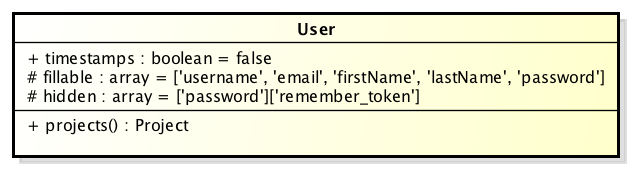
\includegraphics[width=0.5\linewidth]{img/User}
		\caption[Diagramma della classe User]{Diagramma della classe User}
	\end{figure}

	\paragraph{Descrizione}
	Il model User permette di gestire la collection users del database. Eloquent presume che il nome della classe sia il singolare del nome della collection nel database, quindi collega User alla collection users.
	
	\paragraph{Utilizzo}
	Il model gestisce la collection users del database.
	
	\paragraph{Attributi}
	\begin{itemize}
		\item \textbf{+ timestamps : boolean = false :}\\
		Di default Eloquent automatizza l'inserimento del timestamp relativo all'inserimento e aggiornamento di un campo. Se alla variabile viene assegnato il valore le informazioni dell'inserimento e del aggiornamento non verranno aggiunto alla collection.
		\item \textbf{\# fillable : array = ['username', 'email', 'firstName', 'lastName', 'password']:}\\
		Quando si crea un model, si deve passare una serie di attributi al costruttore del model stesso. Questi attributi vengono assegnati al model tramite \textbf{mass assignment}. La propietà \textit{fillable} serve a specificare quali attributi devono essere assegnabili tramite il mass-assignment.
		\item \textbf{\# hiddem : array = ['password', 'remember\_token''] : }\\
		La proprietà hidden si aggiunge quando si vuole limitare gli attributi che sono inclusi nel JSON.
	\end{itemize}
	
	\paragraph{Metodi}
	\begin{itemize}
		\item \textbf{+ projects() : Project}\\
		Abbiamo utilizzato la relazione embedsMany per riuscire ad incorporare il model projects all'interno dell'oggetto principale User. Il metodo ritorna Project su cui verrà chiamato il metodo save() nel caso in cui si voglia aggiornare il modello.
	\end{itemize}